\documentclass{report}
\usepackage{graphicx, tikz-cd, float, titlepic, booktabs} % Required for inserting images
\usepackage{pgfplots}
\usepackage{multicol}
\usepackage{makecell}
\pgfplotsset{compat=1.15}
\usepackage{mathrsfs}
\usetikzlibrary{arrows}
\usepackage{amsmath, amssymb, amsthm, amsfonts, siunitx, physics, gensymb}
\AtBeginDocument{\RenewCommandCopy\qty\SI}
\usepackage[version=4]{mhchem}
\usepackage[most,many,breakable]{tcolorbox}
\usepackage{xcolor, fancyhdr, varwidth}
\usepackage[Glenn]{fncychap}
%Options: Sonny, Lenny, Glenn, Conny, Rejne, Bjarne, Bjornstrup
\usepackage{hyperref, cleveref}
\usepackage{icomma, enumitem} %comma as decimal and continue enumerate with [resume]
\usepackage{plimsoll} %use standard state symbol with \stst
\usepackage[danish]{babel}
\renewcommand{\cellalign}{cl}
\renewcommand{\theadalign}{cl}
\renewcommand\theadfont{\bfseries}
%%%%%%%%%%%%%%%%%%%%%%%%%%%%%%
% SELF MADE COLORS
%%%%%%%%%%%%%%%%%%%%%%%%%%%%%%
\definecolor{myg}{RGB}{56, 140, 70}
\definecolor{myb}{RGB}{45, 111, 177}
\definecolor{myr}{RGB}{199, 68, 64}
\definecolor{mytheorembg}{HTML}{F2F2F9}
\definecolor{mytheoremfr}{HTML}{00007B}
\definecolor{mylenmabg}{HTML}{FFFAF8}
\definecolor{mylenmafr}{HTML}{983b0f}
\definecolor{mypropbg}{HTML}{f2fbfc}
\definecolor{mypropfr}{HTML}{191971}
\definecolor{myexamplebg}{HTML}{F2FBF8}
\definecolor{myexamplefr}{HTML}{88D6D1}
\definecolor{myexampleti}{HTML}{2A7F7F}
\definecolor{mydefinitbg}{HTML}{E5E5FF}
\definecolor{mydefinitfr}{HTML}{3F3FA3}
\definecolor{notesgreen}{RGB}{0,162,0}
\definecolor{myp}{RGB}{197, 92, 212}
\definecolor{mygr}{HTML}{2C3338}
\definecolor{myred}{RGB}{127,0,0}
\definecolor{myyellow}{RGB}{169,121,69}
\definecolor{myexercisebg}{HTML}{F2FBF8}
\definecolor{myexercisefg}{HTML}{88D6D1}
%%%%%%%%%%%%%%%%%%%%%%%%%%%%%%%%%%%%%%%%%%%%%%%%%%%%%%%%%%%%%%%%%%%%%%
% Box environments for theorems and problems
%%%%%%%%%%%%%%%%%%%%%%%%%%%%%%%%%%%%%%%%%%%%%%%%%%%%%%%%%%%%%%%%%%%%%
\setlength{\parindent}{1cm}
%================================
% Question BOX
%================================
\makeatletter
\newtcbtheorem{question}{Opgave}{enhanced,
	breakable,
	colback=white,
	colframe=myb!80!black,
	attach boxed title to top left={yshift*=-\tcboxedtitleheight},
	fonttitle=\bfseries,
	title={#2},
	boxed title size=title,
	boxed title style={%
			sharp corners,
			rounded corners=northwest,
			colback=tcbcolframe,
			boxrule=0pt,
		},
	underlay boxed title={%
			\path[fill=tcbcolframe] (title.south west)--(title.south east)
			to[out=0, in=180] ([xshift=5mm]title.east)--
			(title.center-|frame.east)
			[rounded corners=\kvtcb@arc] |-
			(frame.north) -| cycle;
		},
	#1
}{def}
\makeatother
%================================
% DEFINITION BOX
%================================

\newtcbtheorem[number within=section]{definition}{Definition}{enhanced,
	before skip=2mm,after skip=2mm, colback=red!5,colframe=red!80!black,boxrule=0.5mm,
	attach boxed title to top left={xshift=1cm,yshift*=1mm-\tcboxedtitleheight}, varwidth boxed title*=-3cm,
	boxed title style={frame code={
					\path[fill=tcbcolback]
					([yshift=-1mm,xshift=-1mm]frame.north west)
					arc[start angle=0,end angle=180,radius=1mm]
					([yshift=-1mm,xshift=1mm]frame.north east)
					arc[start angle=180,end angle=0,radius=1mm];
					\path[left color=tcbcolback!60!black,right color=tcbcolback!60!black,
						middle color=tcbcolback!80!black]
					([xshift=-2mm]frame.north west) -- ([xshift=2mm]frame.north east)
					[rounded corners=1mm]-- ([xshift=1mm,yshift=-1mm]frame.north east)
					-- (frame.south east) -- (frame.south west)
					-- ([xshift=-1mm,yshift=-1mm]frame.north west)
					[sharp corners]-- cycle;
				},interior engine=empty,
		},
	fonttitle=\bfseries,
	title={#2},#1}{def}

%================================
% NOTE BOX
%================================

\usetikzlibrary{arrows,calc,shadows.blur}
\tcbuselibrary{skins}
\newtcolorbox{note}[1][]{%
	enhanced jigsaw,
	colback=gray!20!white,%
	colframe=gray!80!black,
	size=small,
	boxrule=1pt,
	title=\textbf{Note:},
	halign title=flush center,
	coltitle=black,
	breakable,
	drop shadow=black!50!white,
	attach boxed title to top left={xshift=1cm,yshift=-\tcboxedtitleheight/2,yshifttext=-\tcboxedtitleheight/2},
	minipage boxed title=1.5cm,
	boxed title style={%
			colback=white,
			size=fbox,
			boxrule=1pt,
			boxsep=2pt,
			underlay={%
					\coordinate (dotA) at ($(interior.west) + (-0.5pt,0)$);
					\coordinate (dotB) at ($(interior.east) + (0.5pt,0)$);
					\begin{scope}
						\clip (interior.north west) rectangle ([xshift=3ex]interior.east);
						\filldraw [white, blur shadow={shadow opacity=60, shadow yshift=-.75ex}, rounded corners=2pt] (interior.north west) rectangle (interior.south east);
					\end{scope}
					\begin{scope}[gray!80!black]
						\fill (dotA) circle (2pt);
						\fill (dotB) circle (2pt);
					\end{scope}
				},
		},
	#1,
}
%================================
% EXAMPLE BOX
%================================
\newtcbtheorem[number within=section, use counter from=definition]{Example}{Example}
{%
	colback = myexamplebg
	,breakable
	,colframe = myexamplefr
	,coltitle = myexampleti
	,boxrule = 1pt
	,sharp corners
	,detach title
	,before upper=\tcbtitle\par\smallskip
	,fonttitle = \bfseries
	,description font = \mdseries
	,separator sign none
	,description delimiters parenthesis
}
{ex}
%================================
% THEOREM BOX
%================================

\tcbuselibrary{theorems,skins,hooks}
\newtcbtheorem[number within=section, use counter from=definition]{Theorem}{Theorem}
{%
	enhanced,
	breakable,
	colback = mytheorembg,
	frame hidden,
	boxrule = 0sp,
	borderline west = {2pt}{0pt}{mytheoremfr},
	sharp corners,
	detach title,
	before upper = \tcbtitle\par\smallskip,
	coltitle = mytheoremfr,
	fonttitle = \bfseries\sffamily,
	description font = \mdseries,
	separator sign none,
	segmentation style={solid, mytheoremfr},
}
{th}

%%%%%%%%%%%%%%%%%%%%%%%%%%%%%%%%%%%%%%%%%%%%%%%%%%%%%%%%%%%%%%%%%
% SELF MADE COMMANDS
%%%%%%%%%%%%%%%%%%%%%%%%%%%%%%
\newcommand{\sol}{\setlength{\parindent}{0cm}\textbf{\textit{Løsning:}}\setlength{\parindent}{1cm}}
%%%%%%%%%%%%%%%%%%%%%%%%%%%%%%%%%
\usepackage[tmargin=2cm,rmargin=1in,lmargin=1in,margin=0.85in,bmargin=2cm,footskip=.2in]{geometry}\pagestyle{fancy}
\lhead{Fysik A}
\rhead{Terminsprøve}

\title{Terminsprøve\\
{\Large \textbf{Fysik A}}}
\date{\today}

\begin{document}
\maketitle
\begin{note}
  Databog fysik kemi (2007) er benyttet ved beregningerne.
\end{note}
\section*{Opgave 1: Varme glas}
\sol \\
\textbf{a.}
Varmekapaciteten er blot produktet af den specifikke varmekapacitet og massen.
\begin{equation*}
\begin{split}
  C&=m \cdot c \\
  &=0,170 \;\unit{kg} \cdot 840 \;\unit{\frac{J}{kg \cdot K}} \\
  &\approx 143 \;\unit{J/K} 
\end{split}
\end{equation*}
Varmekapaciteten af et glas er altså $143 \;\unit{J/K} $.\\[1ex]
\textbf{b.}
Vi antager, at glasset med vandet er et isoleret system.
Der gælder så
\begin{equation*}
\begin{split}
  \Delta E=0 &\iff \Delta E_{\text{glas} } + \Delta E _{\text{vand} }=0\\
  &\iff m_{\text{glas} } \cdot c_{\text{glas} } \cdot \Delta T_{\text{glas} } + m_{\text{vand} } \cdot c_{\text{vand} } \cdot \Delta T_{\text{vand} }=0\\
  &\iff m_{\text{glas} } \cdot c_{\text{glas} } \cdot \left(T _{\text{slut} }-T _{\text{glas} }\right) + m_{\text{vand} } \cdot c_{\text{vand} } \cdot \left(T _{\text{slut} }-T _{\text{vand} }\right)=0\\
  &\iff T _{\text{slut} }=\frac{m_{\text{glas} } \cdot c_{\text{glas} } \cdot T _{\text{glas} }+m_{\text{vand} } \cdot c_{\text{vand} } \cdot T _{\text{vand} }}{m_{\text{glas} } \cdot c_{\text{glas} } + m_{\text{vand} } \cdot c_{\text{vand} }}
\end{split}
\end{equation*}
Vi indsætter de kendte værdier og udregner da temperaturen til slut.
\begin{equation*}
\begin{split}
  T _{\text{slut} }&=\frac{m_{\text{glas} } \cdot c_{\text{glas} } \cdot T _{\text{glas} }+m_{\text{vand} } \cdot c_{\text{vand} } \cdot T _{\text{vand} }}{m_{\text{glas} } \cdot c_{\text{glas} } + m_{\text{vand} } \cdot c_{\text{vand} }}\\
  &=\frac{0,170 \;\unit{kg} \cdot 840 \;\unit{\frac{J}{kg \cdot K}} \cdot 42 \;\unit{\celsius} + 0,210 \;\unit{kg} \cdot 4,182 \cdot 10^3\;\unit{\frac{J}{kg \cdot K}} \cdot 5 \;\unit{\celsius} }{0,170 \;\unit{kg} \cdot 840 \;\unit{\frac{J}{kg \cdot K}} + 0,210 \;\unit{kg} \cdot 4,182 \cdot 10^3\;\unit{\frac{J}{kg \cdot K}}}\\
  &\approx 10 \;\unit{\celsius} 
\end{split}
\end{equation*}
Når der er termisk ligevægt bliver temperaturen af vandet altså $10 \;\unit{\celsius} $.
\section*{Opgave 2: Ganymedes}
\sol \\
\textbf{a.}
Vi antager, at Ganymedes har form som en bold.
Et udtryk for Ganymedes volumen bliver så 
\begin{equation*}
\begin{split}
  V&=\frac{4}{3} \cdot \pi  \cdot \left(\frac{1}{2} d\right)^{3}\\
  &=\frac{1}{6} \cdot \pi \cdot d^3
\end{split}
\end{equation*}
Da densitet er masse per volumen, får vi så
\begin{equation*}
\begin{split}
  \rho &=\frac{m}{V}\\
  &=\frac{6 \cdot m}{ \pi \cdot  d ^3}\\
  &=\frac{6 \cdot 1,482 \cdot 10 ^{23} \;\unit{kg} }{ \pi \cdot \left(5262 \cdot 10^3 \;\unit{m} \right) ^3 }\\
  &\approx 1943 \;\unit{kg/m^3} 
\end{split}
\end{equation*}
Densiteten af Ganymedes er altså $1943 \;\unit{kg/m^3} $.\\[1ex]
\textbf{b.}
Vi lader $M$ betegne Ganymedes masse, og $r$ betegne afstanden fra Ganymedes massemidtpunkt (her centrum) til dens overflade.
Så gælder der fra gravitationsloven, at 
\begin{equation*}
\begin{split}
  a _{\text{tyngde} }&=\frac{F _{G}}{m}\\
  &=G \cdot \frac{M}{r^2}\\
  &=G \cdot \frac{M}{\left(\frac{1}{2}d\right) ^2}\\
  &=G \cdot \frac{4 \cdot M}{d^2}\\
  &=6,674 \cdot 10 ^{-11} \;\unit{\frac{N \cdot m^2}{kg^2}} \cdot \frac{4 \cdot 1,482 \cdot 10 ^{23}\;\unit{kg} }{\left(5262 \cdot 10^3 \;\unit{m} \right) ^2}\\
  &\approx 1,429 \;\unit{m/s^2} 
\end{split}
\end{equation*}
Tyngdeaccelerationen på overfladen af Ganymedes er altså $1,429 \;\unit{m/s^2} $.\\[1ex]
\textbf{c.}
Vi antager, at der er tale om en jævn cirkelbevægelse.
Afstanden fra sonden til Ganymedes' overflade betegner vi $s$, og accelerationen da være
\begin{equation*}
\begin{split}
  a&=\frac{v^2}{\left(\frac{1}{2}d + s\right) }\\
  &=\frac{4 \cdot \pi ^2}{T^2}\cdot \left(\frac{1}{2}d + s\right) 
\end{split}
\end{equation*}
Denne acceleration mod Ganymedes (som er centrum for bevægelsen), må komme fra tyngdeaccelerationen.
 der gælder
\begin{equation*}
\begin{split}
  a=\frac{4 \cdot \pi ^2}{T^2}\cdot \left(\frac{1}{2}d + s\right)  = G \cdot \frac{M}{\left( \frac{1}{2}d + s\right)^2} &\iff \left(\frac{1}{2}d + s\right) ^3=\frac{G \cdot M \cdot T^2}{4 \cdot \pi ^2}\\
  &\iff s=\sqrt[3]{\frac{G \cdot M \cdot T^2}{4 \cdot \pi ^2}} - \frac{1}{2}d
\end{split}
\end{equation*}
Vi indsætter de kendte værdier og beregner afstanden $s$.
\begin{equation*}
\begin{split}
  s&=\sqrt[3]{\frac{G \cdot M \cdot T^2}{4 \cdot \pi ^2}} - \frac{1}{2}d\\
  &=\sqrt[3]{\frac{6,674 \cdot 10 ^{-11} \;\unit{\frac{N \cdot m^2}{kg^2}} \cdot 1,482 \cdot 10 ^{23}\;\unit{kg} \cdot \left(8 \cdot 60^2 \;\unit{s}  + 30 \cdot 60 \;\unit{s} \right)^2}{4 \cdot \pi ^2}} - \frac{1}{2} \cdot 5262 \cdot 10^3 \;\unit{m} \\
  &\approx 3536 \cdot 10^3 \;\unit{m} \\
  &=3536 \;\unit{km} 
\end{split}
\end{equation*}
Rumsonden befinder sig altså 3536 km over Ganymedes' overflade.
\section*{Opgave 3: Elcykel}
\sol \\
\textbf{a.}
Vi aflæser på $(v,P)$-grafen (se \cref{fig:vP}), at når cyklen kører med $35 \;\unit{km/t} $, så er effekten $P=575 \;\unit{W} $.
Vi finder nu et udtryk for strømstyrken udtrykt ved effekten og spændingsfaldet.
\begin{equation*}
\begin{split}
  P=U \cdot I \iff I=\frac{P}{U}
\end{split}
\end{equation*}
Vi udregner nu strømstyrken $I$.
\begin{equation*}
\begin{split}
  I&=\frac{P}{U}\\
  &=\frac{575 \;\unit{W} }{36 \;\unit{V} }\\
  &\approx 16 \;\unit{A} 
\end{split}
\end{equation*}
Når cyklen kører med $35 \;\unit{km/t} $, så er strømstyrken gennem motoren altså $16 \;\unit{A} $.
\begin{figure}[H]
\begin{center}
  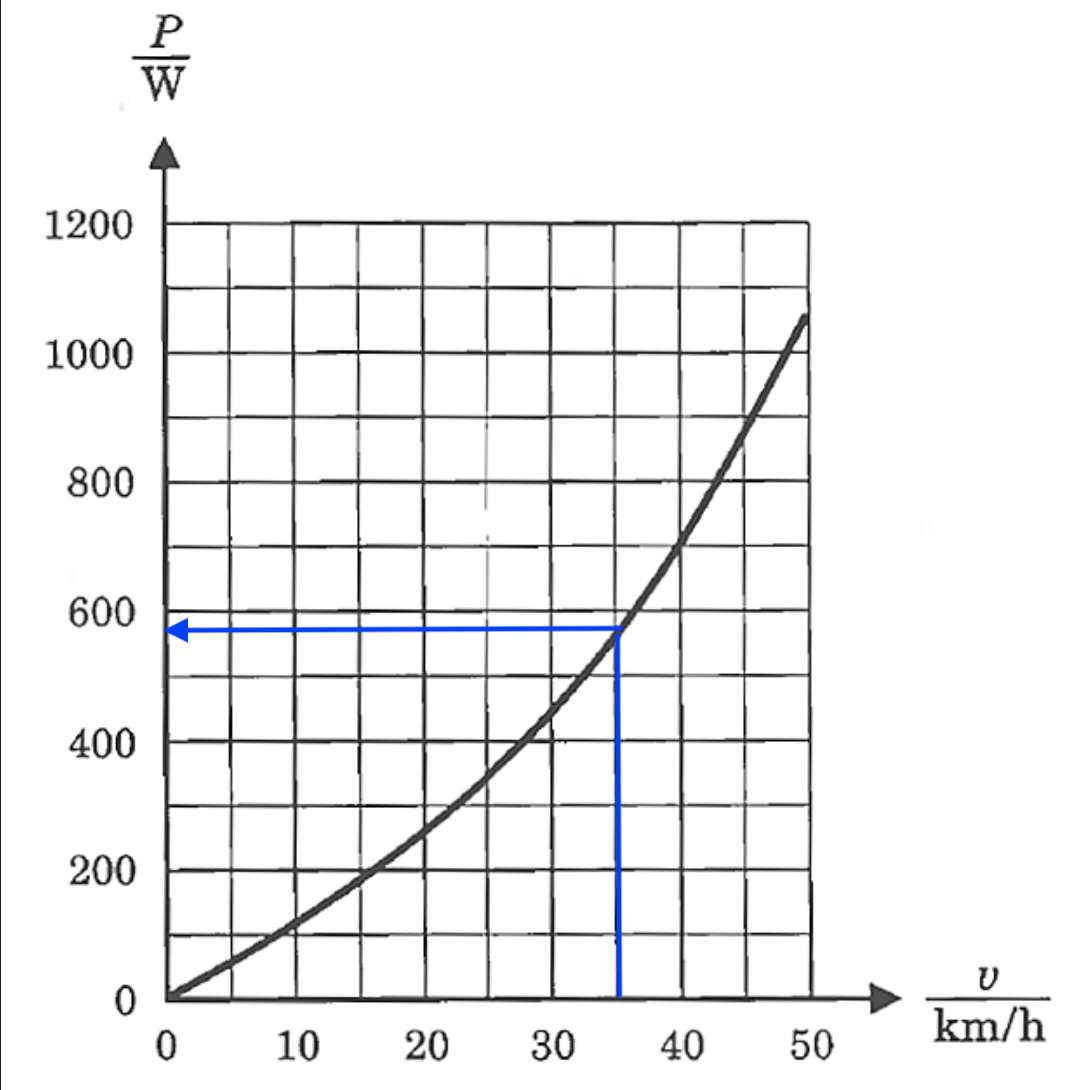
\includegraphics[width=0.5\textwidth]{vP.png}
\end{center}
  \caption{Aflæsning på $(v,P)$-grafen for cyklens motor}
\label{fig:vP}
\end{figure}
\noindent \textbf{b.}
Vi aflæser på $(v,P)$-grafen (se \cref{fig:vP30}), at når cyklen kører med $30 \;\unit{km/t} $, så er effekten $P=450 \;\unit{W} $.
\begin{figure}[H]
\begin{center}
  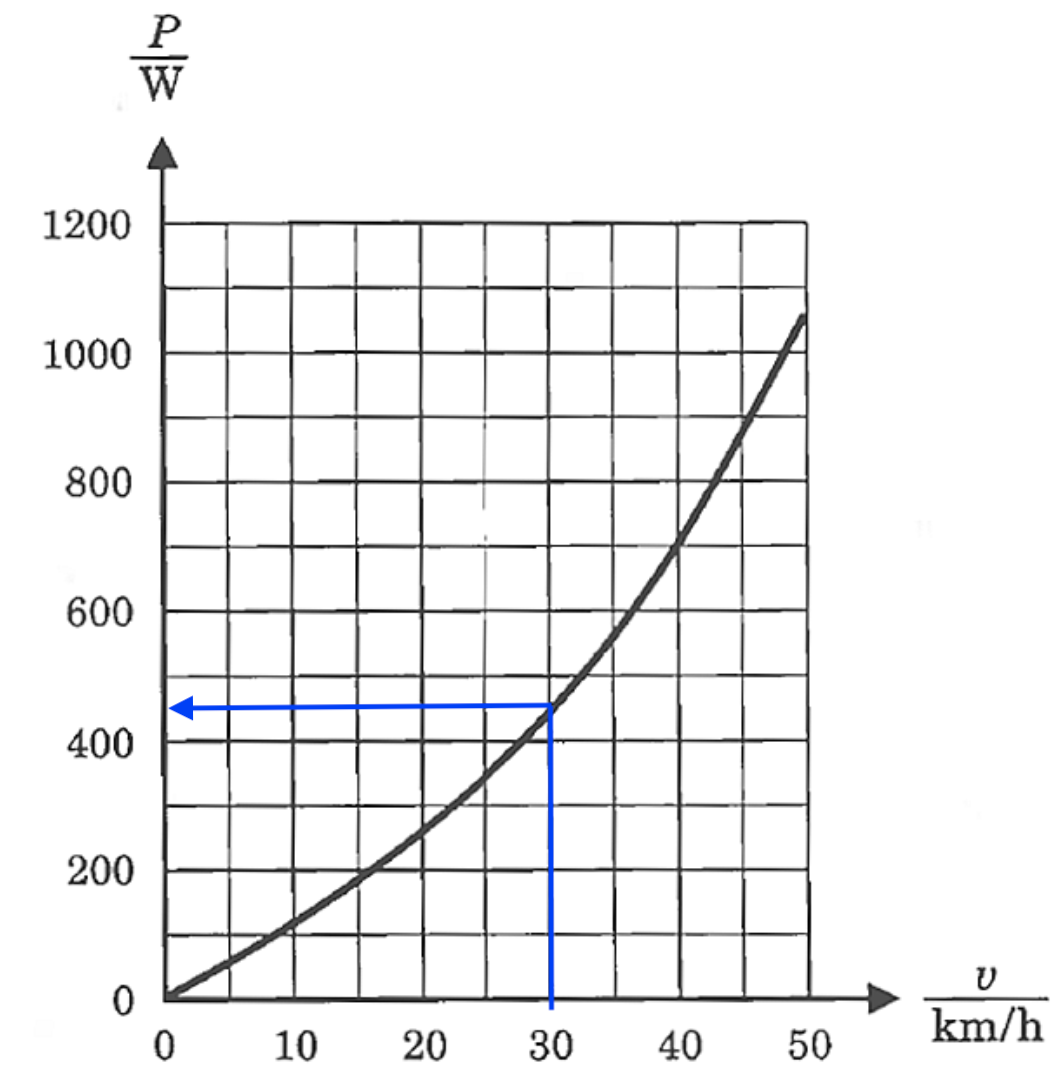
\includegraphics[width=0.4\textwidth]{vP30.png}
\end{center}
  \caption{Aflæsning på $(v,P)$-grafen for cyklens motor}
\label{fig:vP30}
\end{figure}

Vi starter med at omregne tiden til sekunder.
\begin{equation*}
\begin{split}
  t&=2 \;\unit{t} \\
  &=2 \cdot 60^2 \;\unit{s} \\
  &=7200 \;\unit{s} 
\end{split}
\end{equation*}
Vi kan nu udregne energien, som batteriet afgiver på de to timer.
\begin{equation*}
\begin{split}
  E&=P \cdot t \\
  &=450 \;\unit{W} \cdot 7200 \;\unit{s} \\
  &\approx 3 \cdot 10 ^{6}\;\unit{J} \\
  &=3 \;\unit{MJ} 
\end{split}
\end{equation*}
Energien, som batteriet kan afgive er altså $3 \;\unit{MJ} $. \\[1ex]
\textbf{c.}
Vi aflæser på $(v,P)$-grafen (se \cref{fig:vP40}), at når cyklen kører med $40 \;\unit{km/t} $, så er effekten $P=700 \;\unit{W} $.
\begin{figure}[H]
\begin{center}
  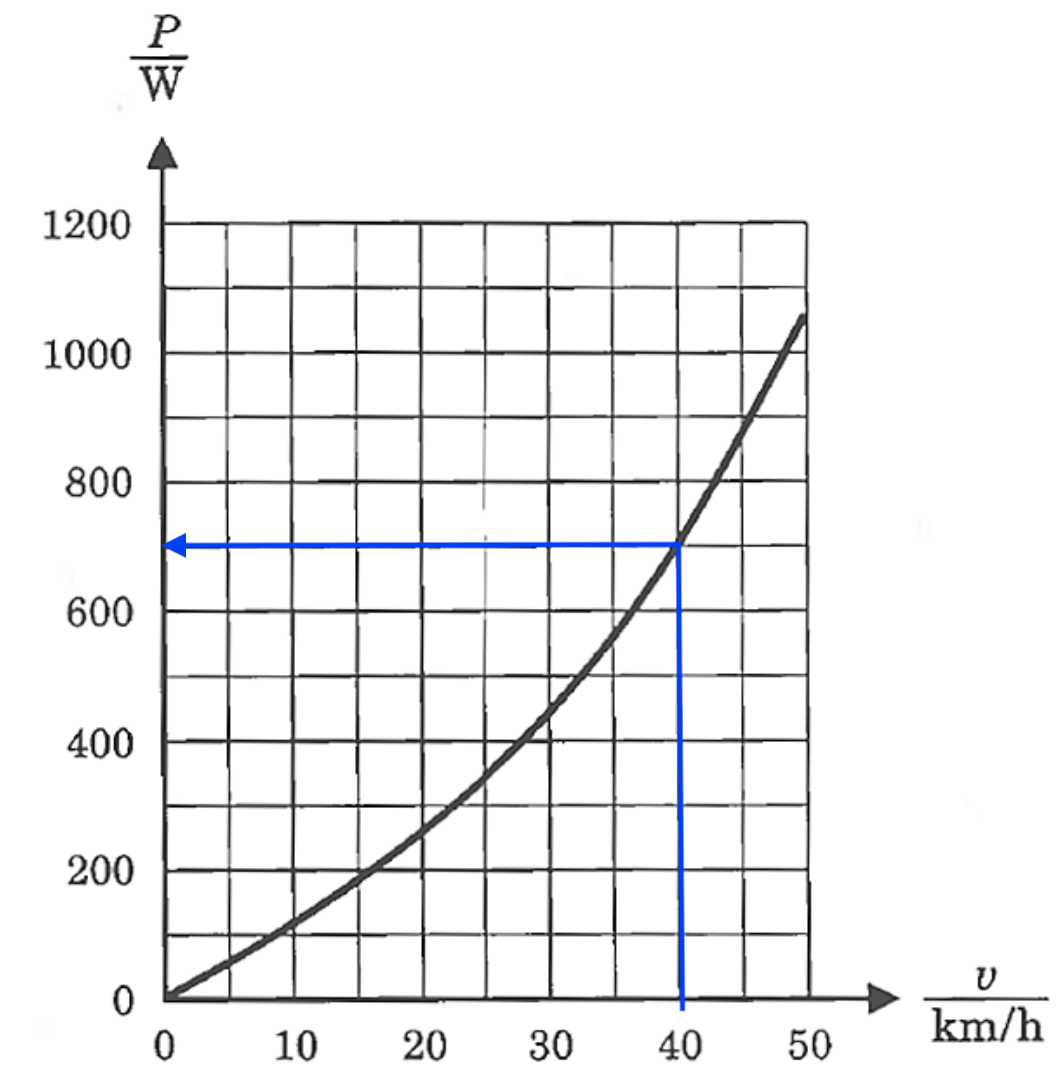
\includegraphics[width=0.5\textwidth]{vP40.png}
\end{center}
  \caption{Aflæsning på $(v,P)$-grafen for cyklens motor}
\label{fig:vP40}
\end{figure}
Vi finder et udtryk for tiden, som cyklen kan køre med $40 \;\unit{km/t} $.
\begin{equation*}
\begin{split}
  P=\frac{E}{t} \iff t=\frac{E}{P}
\end{split}
\end{equation*}
Lad $s$ være afstanden, som cyklen kan køre med $40 \;\unit{km/t} $.
Så må der, siden der er tale om en bevægelse med konstant fart, gælde
\begin{equation*}
\begin{split}
  s&=v \cdot t \\
  &=v \cdot \frac{E}{P}\\
  &=40 \;\unit{km/t} \cdot \frac{3,24 \cdot 10 ^{6}\;\unit{J} }{700 \;\unit{W} }\\
  &=\frac{40}{3,6} \;\unit{m/s} \cdot \frac{3,24 \cdot 10 ^{6}\;\unit{J} }{700 \;\unit{W} }\\
  &\approx 5,1 \cdot 10^4 \;\unit{m} \\
  &=51 \;\unit{km} 
\end{split}
\end{equation*}
Cyklen kan altså køre $51 \;\unit{km} $ med farten $40 \;\unit{km/t} $ på en fuld opladning. 
\section*{Opgave 4: Malingsryster}
\sol \\
\textbf{a.}
Der gælder for harmoniske svingninger, at svingningstiden for accelerationen er den samme som svingningstiden for positionen (for at se hvorfor, tænk på, hvad der sker, når man differentierer de trigonometriske funktioner $\cos$ og $\sin$).
Vi aflæser på $(t,a)$-grafen (se \cref{fig:ta}), at svingningstiden for accelerationen er $0,09 \;\unit{s} $.

Altså må svingningstiden for spanden også være $0,09 \;\unit{s} $.
\begin{figure}[H]
\begin{center}
  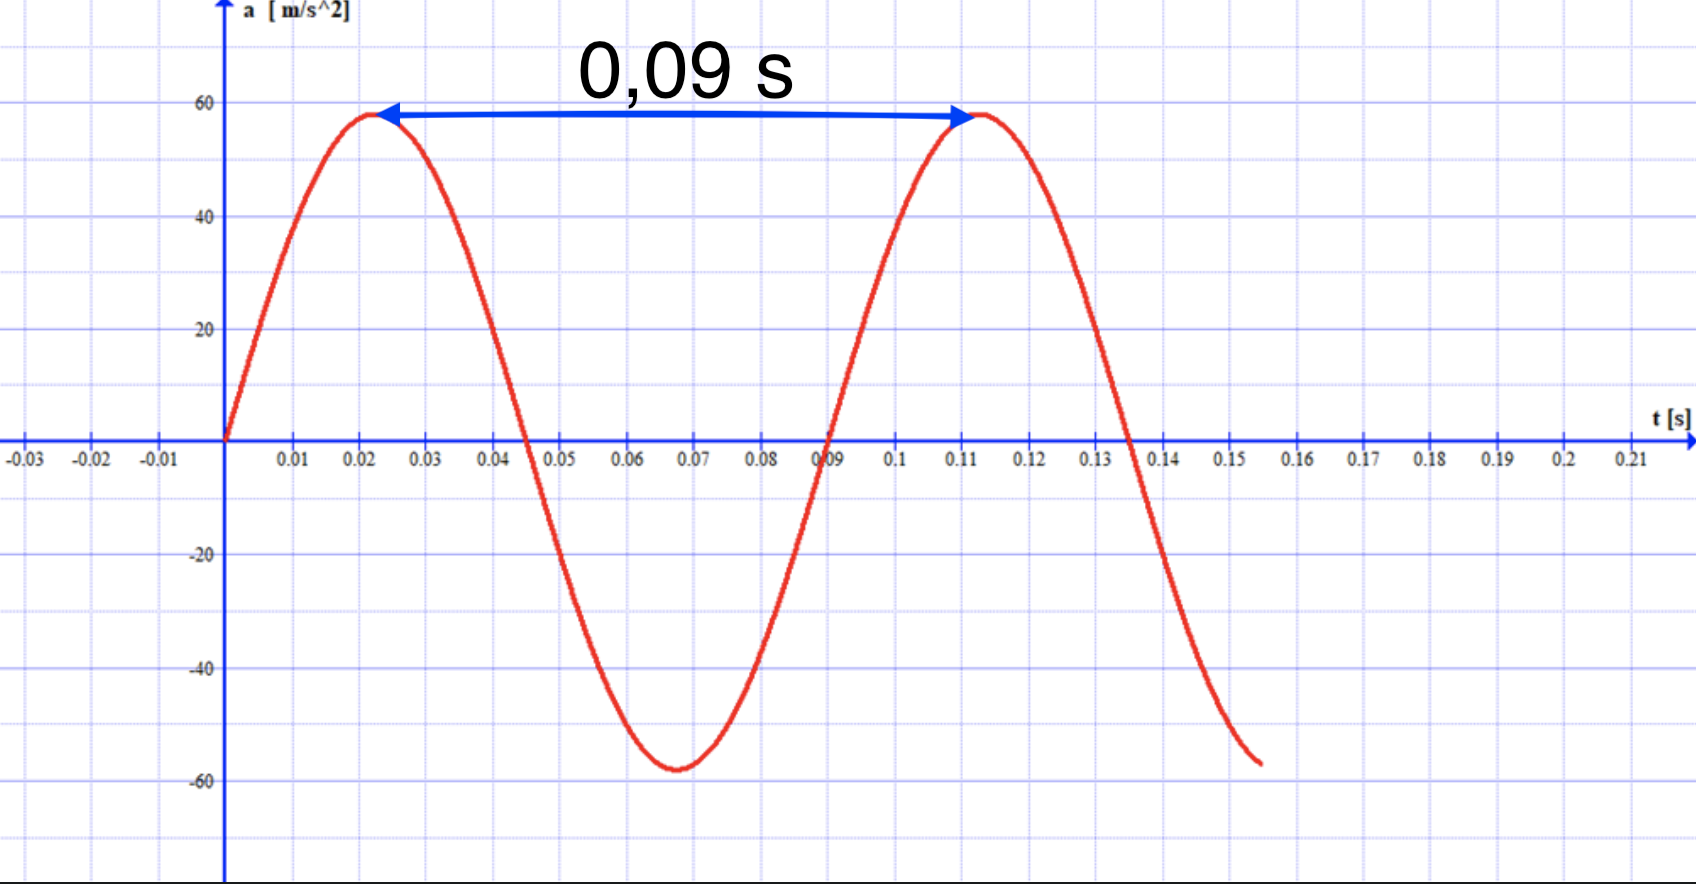
\includegraphics[width=0.7\textwidth]{ta.png}
\end{center}
  \caption{Aflæsning på $(t,a)$-grafen for spanden}
\label{fig:ta}
\end{figure}
\noindent \textbf{b.}
Siden sammenhængen mellem farten $v$ og accelerationen $a$ er 
\begin{equation*}
\begin{split}
  \Delta v = \int_{t_1}^{t_2} a(t) \,dt 
\end{split}
\end{equation*}
og spanden er i hvile til start, så må $v$ svare til det samlede areal under $(t,A)$-grafen (hvor areal under $t$-aksen tæller negativt).
Spanden må da nå sin maksimale fart, når grafen skærer $t$-aksen med negativ hældning.
Vi finder antallet af tern under grafen første gang dette sker, hvilket gøres med en billedeanalyse i Logger Pro, som ses i \cref{fig:tareal} (det antages, at ternene er kvadratiske).
\begin{figure}[H]
\begin{center}
  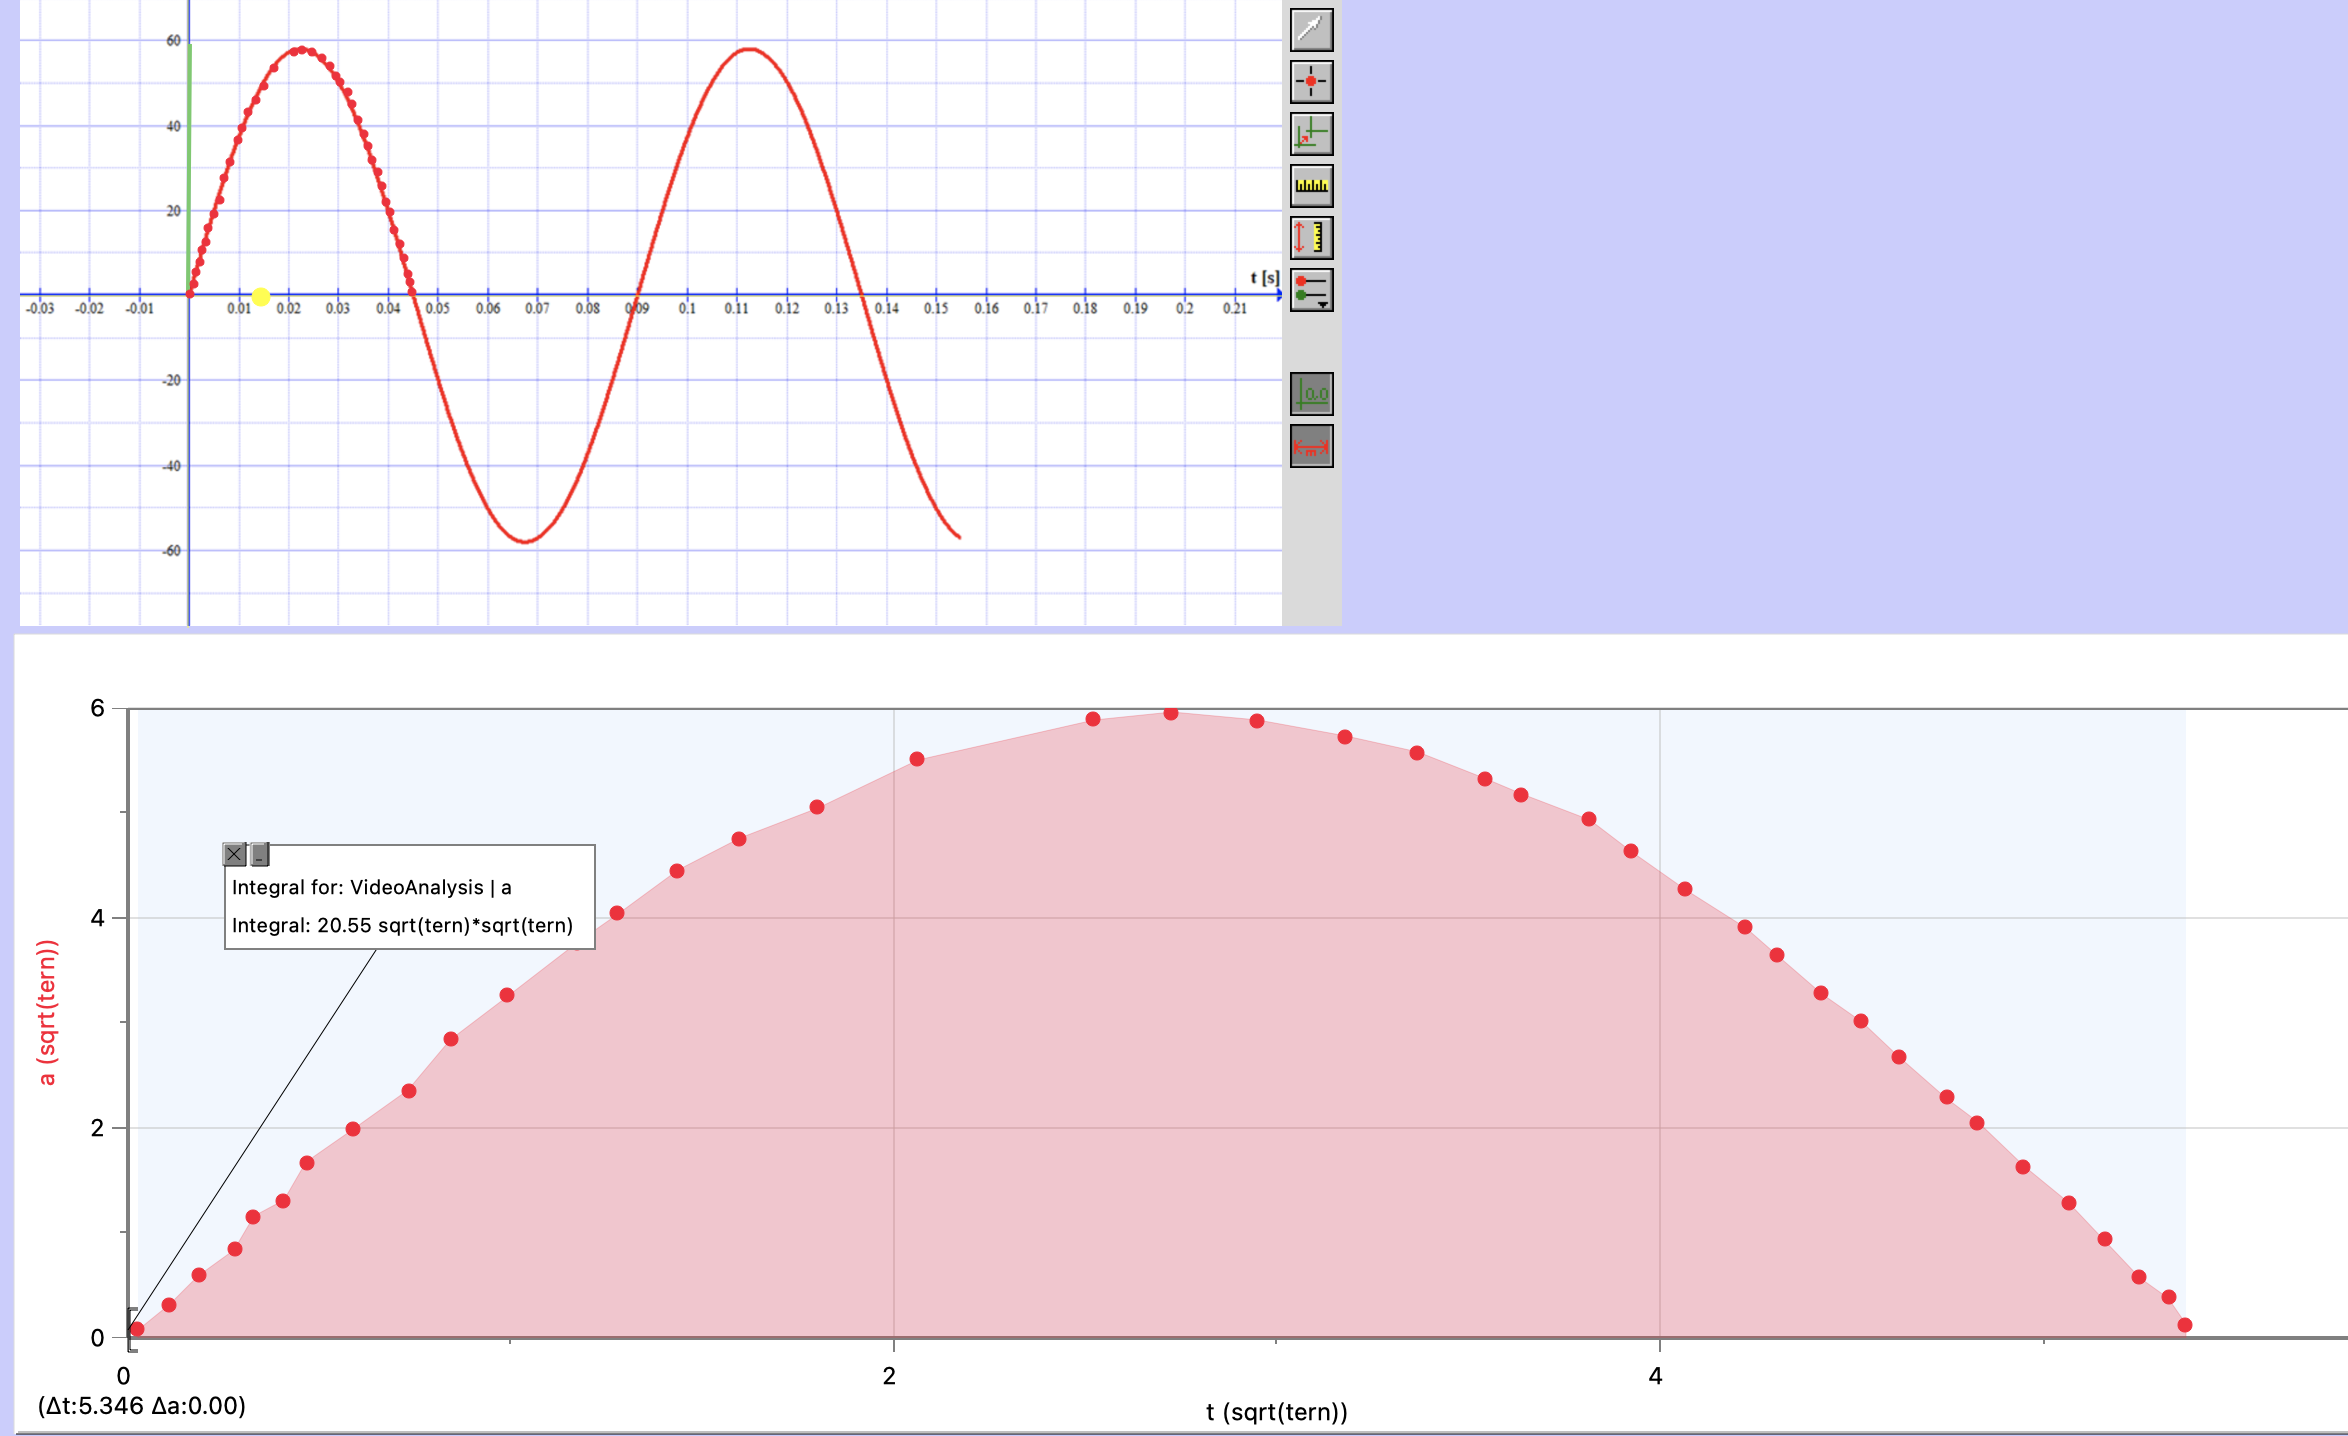
\includegraphics[width=0.6\textwidth]{tareal.png}
\end{center}
\caption{Antal tern under første del af $(t,A)$-grafen fundet med Logger Pro}
\label{fig:tareal}
\end{figure}
Fra billedeanalysen har vi, at det samlede antal tern under grafen når den skærer $t$-aksen er $20,55$.
Hvert tern svarer til
\[
0,01 \;\unit{s}  \cdot 10 \;\unit{m/s^2} =0,1 \;\unit{m/s} 
\] 
Spandens maksimale fart må da være
\begin{equation*}
\begin{split}
20,55 \cdot 0,1 \;\unit{m/s} \approx 2,05 \;\unit{m/s} 
\end{split}
\end{equation*}
Spandens maksimale fart i lodret retning er altså $2,05 \;\unit{m/s} $.\\[1ex]
\textbf{c.}
Fra Newtons anden lov er det klart, at størrelsen af den lodrette kraft på spanden er maksimal når størrelsen af den lodrette acceleration er maksimal:
\begin{equation*}
\begin{split}
  F=m \cdot a
\end{split}
\end{equation*}
Vi aflæser, at den maksimale størrelse af den lodrette acceleration på spanden er $58 \;\unit{m/s^2} $.
Vi udregner nu størrelsen af den tilsvarende kraft.
\begin{equation*}
\begin{split}
  F&=m \cdot a \\
  &=8,11 \;\unit{kg} \cdot 58 \;\unit{m/s^2} \\
  &\approx 470 \;\unit{N} 
\end{split}
\end{equation*}
Størrelsen af den største kraft i lodret retning fra malingsrysteren på spanden er altså $470 \;\unit{N} $.
\section*{Opgave 5: Varme fra aluminium}
\sol \\
\textbf{a.}
Vi opstiller reaktionsskemaet for $\beta ^+$-henfaldet.
\[
\ce{^26_13Al -> ^26_12Mg + ^0_{+1}e + \nu} 
\] 
For god ordens skyld kontrollerer vi, at ladningen $Z$, nukleontallet $A$ og leptontallet $L$ er bevarede ved reaktionen. 
\begin{equation*}
\begin{split}
  A&: \quad 26 = 26 + 0 + 0 \\
  Z&:\quad 13 = 12 + 1 + 0 \\
  L&:\quad 0 = 0 -1 +1
\end{split}
\end{equation*}
\textbf{b.}
Ved opslag findes halveringstiden af \ce{^26Al} til at være $T _{\frac{1}{2}}=0,72 \;\unit{M} \text{år}  $.\footnote{Databog, s. 200}
Vi lader $N _{0}$ være antallet af \ce{^26Al}-kerner ved jordens dannelse og lader $N$ være antallet af kerner til tiden $t$. 
Så er det oplyst, at
\[
\frac{N}{N _{0}}=0,001
\] 
Vi har så fra henfaldsloven, at
\begin{equation*}
\begin{split}
  \frac{N}{N _{0}}=0,001 = \left(\frac{1}{2}\right) ^{\frac{t}{T _{\frac{1}{2}}}} \iff t = T _{\frac{1}{2}} \cdot \log_{\frac{1}{2}}\left(0,001\right) 
\end{split}
\end{equation*}
Vi beregner nu tiden $t$.
\begin{equation*}
\begin{split}
  t &= T _{\frac{1}{2}} \cdot \log_{\frac{1}{2}}\left(0,001\right)\\
  &=0,72 \;\unit{M} \text{år} \cdot \log_{\frac{1}{2}}\left(0,001\right)\\
  &\approx 7,2 \;\unit{M} \text{år}
\end{split}
\end{equation*}
Der gik altså $7,2 \;\unit{M} \text{år}$ før der kun var 0,1 \% tilbage af det oprindelige \ce{^26Al}.\\[1ex]
\textbf{c.}
Vi beregner først $Q$-værdien for henfaldet af \ce{^26Al}.
\begin{equation*}
\begin{split}
  Q&=-\Delta m \cdot c^2 \\
  &=-\left(\left( m(\ce{^26_12Mg} ) - 12 \cdot m(e)\right) + m(e) - \left(m(\ce{^26_13Al} ) - 13 \cdot m(e)\right) \right) \cdot c^2\\
  &=\left( m(\ce{^26_13Al} ) - m(\ce{^26_12Mg} ) - 2 \cdot m(e)\right) \cdot c^2\\
  &=\left(25,98689169 \;\unit{u} - 25,98259293 \;\unit{u} - 2 \cdot 0,000548580 \;\unit{u} \right) \cdot 931,49 \;\unit{MeV/u} \\
  &\approx 2,9823 \;\unit{MeV} 
\end{split}
\end{equation*}
Fra de givne oplysninger er det klart, at et udtryk for antallet af \ce{^26Al}-kerner til start må være
\begin{equation*}
\begin{split}
  N_0 &=\frac{m _{\text{jord} }\cdot 0,013}{\frac{m(\ce{^26Al} ) + 20000 m(\ce{^27Al} )}{20001}}\\
  &=\frac{m _{\text{jord} }\cdot 0,013 \cdot 20001}{m(\ce{^26Al} ) + 20000 m(\ce{^27Al} )}\\
\end{split}
\end{equation*}
Fra henfaldsloven har vi så, at energien afsat i den første million år må være
\begin{equation*}
\begin{split}
  E&=Q \cdot \Delta N\\
  &=Q \cdot \left(N_0-N\right) \\
  &=Q \cdot N_0 \cdot \left(1-\left(\frac{1}{2}\right) ^{\frac{t}{T _{\frac{1}{2}}}}\right) \\
  &=Q \cdot \frac{m _{\text{jord} }\cdot 0,013 \cdot 20001}{m(\ce{^26Al} ) + 20000 m(\ce{^27Al} )} \cdot \left(1-\left(\frac{1}{2}\right) ^{\frac{t}{T _{\frac{1}{2}}}}\right) \\
  &=2,9823 \;\unit{MeV} \cdot \frac{5,974 \cdot 10 ^{24} \;\unit{kg} \cdot 0,013 \cdot 20001}{25,98689169 \cdot 1,6605 \cdot 10 ^{-27}\;\unit{kg} + 20000 \cdot 26,98153863 \cdot 1,6605 \cdot 10 ^{-27}\;\unit{kg} } \cdot  \left(1-\left(\frac{1}{2}\right) ^{\frac{1 \;\unit{M} \text{år} }{0,72 \;\unit{M} \text{år} }}\right)  \\
  &\approx 
\end{split}
\end{equation*}
ikke tid til at regne ud... skal aflevere nu
\section*{Opgave 6: Trampe}
\sol \\
\textbf{a.}
En videoanalyse laves i Logger Pro, hvilket ses i \cref{fig:video}.
\begin{figure}[H]
\begin{center}
  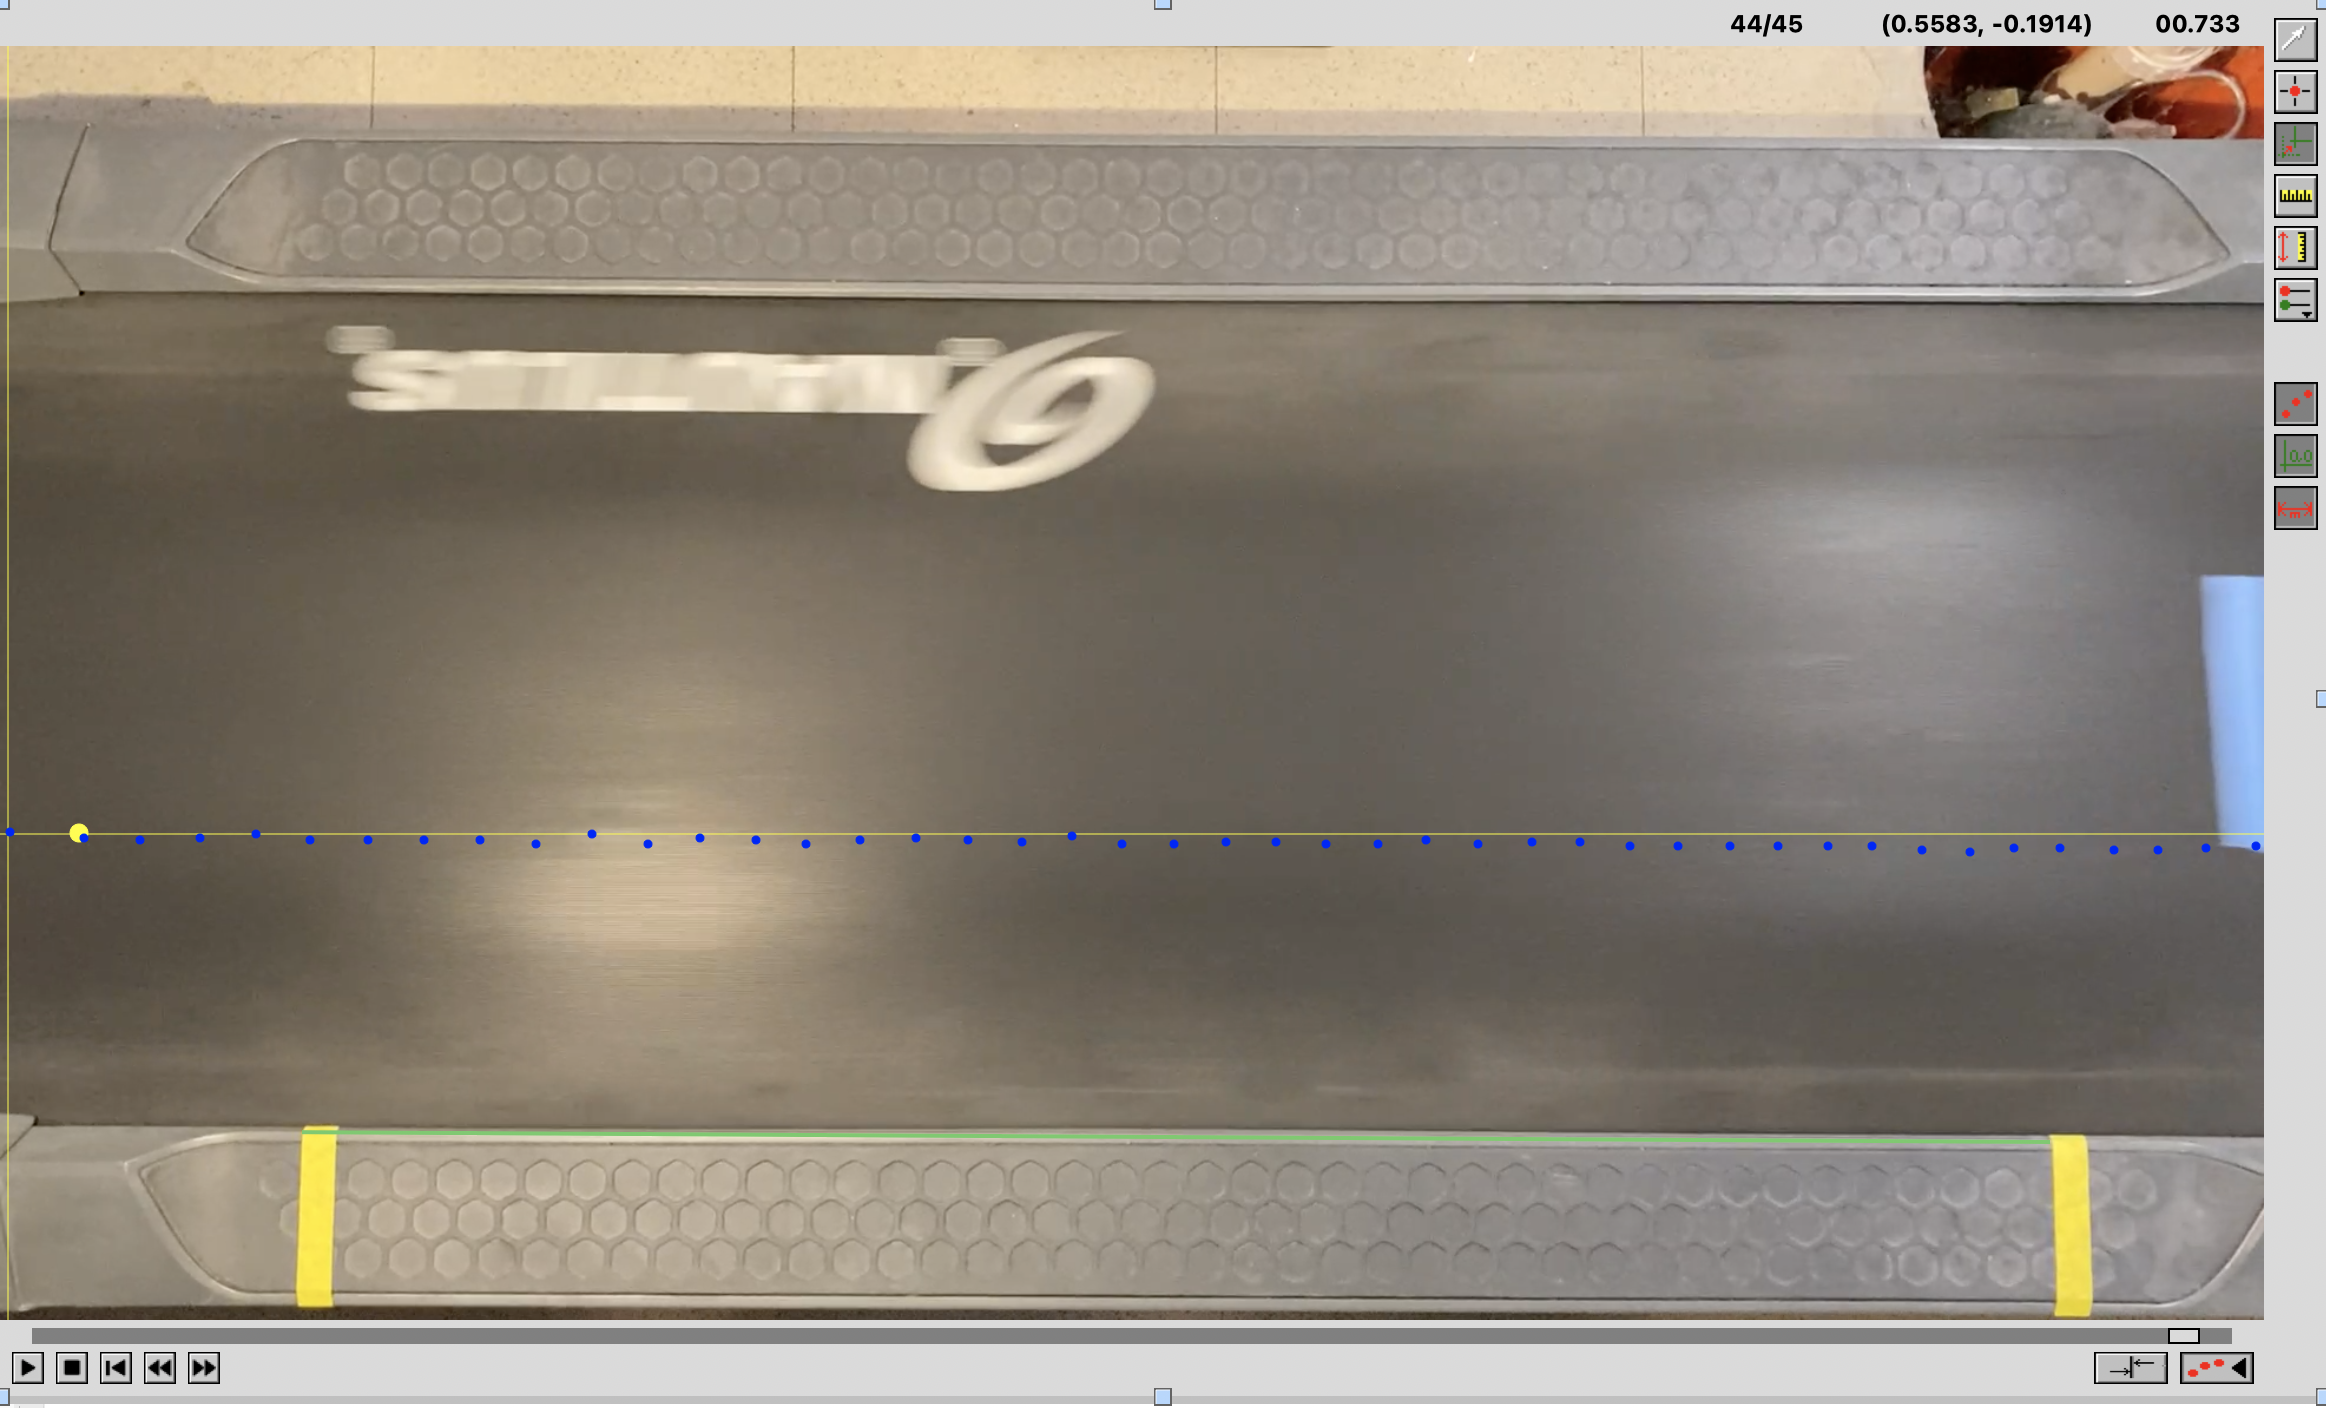
\includegraphics[width=0.7\textwidth]{video.png}
\end{center}
\caption{Videoanalyse laves i Logger Pro}
\label{fig:video}
\end{figure}
Vi antager at der er tale om en bevægelse med konstant fart.
En ny beregnet kolonne laves med den potentielle energi (strengt set er der tale om tilvæksten), som må være
\begin{equation*}
\begin{split}
  E _{\text{pot} }&=m \cdot g \cdot y \\
  &=90 \;\unit{kg} \cdot 9,82 \;\unit{m/s^2} \cdot y \\
  &=883,8 \;\unit{N} \cdot y
\end{split}
\end{equation*}
Siden sammenhængen mellem $E _{\text{pot} }$ og effekten $P$ er 
\[
P=\dv{t} E _{\text{pot} }
\] 
så må hældningen på $(t,E _{\text{pot} })$-grafen være effekten.
Vi tegner da $(t,E _{\text{pot} })$-grafen, og laver lineær regression på punkterne, hvilket ses i \cref{fig:tE}.
\begin{figure}[H]
\begin{center}
  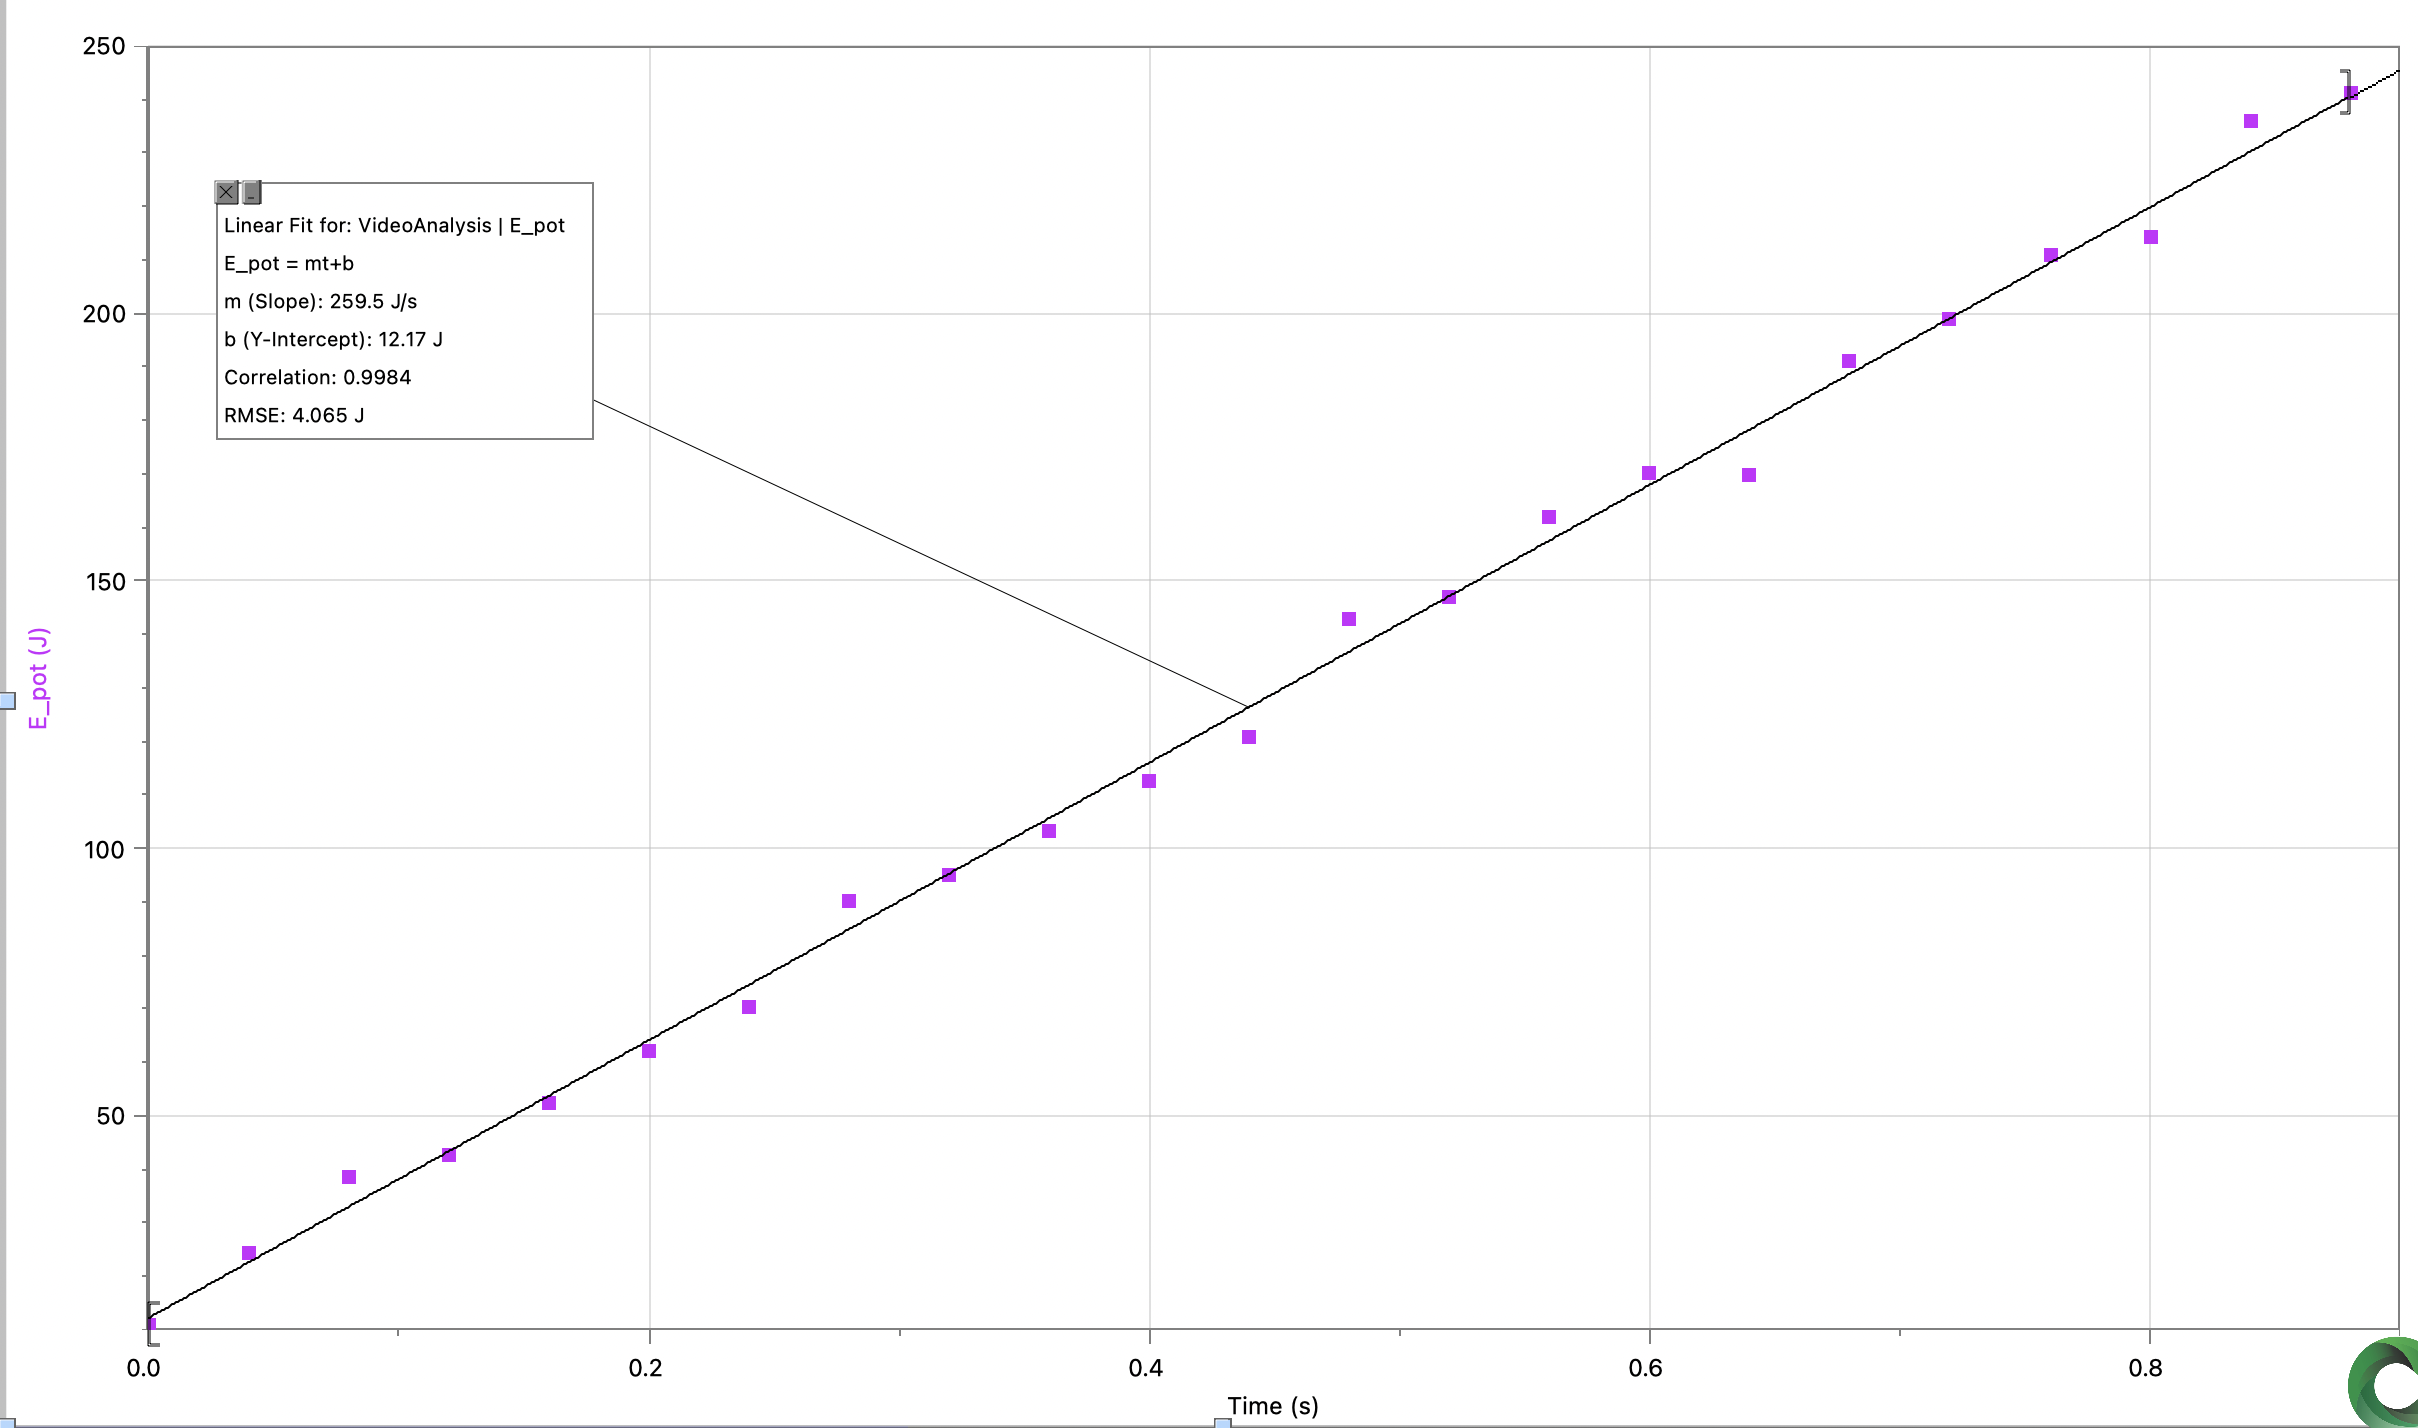
\includegraphics[width=0.7\textwidth]{tE.png}
\end{center}
  \caption{Lineær regression på $(t,E _{\text{pot} })$-grafen lavet i Logger Pro}
\label{fig:tE}
\end{figure}
Fra regressionen har vi, at
\[
P=259,5 \;\unit{W} 
\] 
Effekten, hvormed den potentielle energi for cyklist og cykel øges, når cykelliften skubber cyklisten op ad bakken er altså $259,5 \;\unit{W} $.

\end{document}
